\documentclass{tufte-book}

\usepackage{amsmath, amsthm}
\usepackage{graphicx}
\setkeys{Gin}{width=\linewidth,totalheight=\textheight,keepaspectratio}
\graphicspath{{graphics/}}

\title{STAT 244 \\ Homework 6}
\author{Joe Seidel}
\date{\today}

\usepackage{booktabs}
\usepackage{units}
\usepackage{fancyvrb}
\fvset{fontsize=\normalsize}
\usepackage{multicol}
\usepackage{lipsum}
\usepackage{pdfpages}
\usepackage{tikz}
\usepackage{wasysym}

\newcommand{\doccmd}[1]{\texttt{\textbackslash#1}}% command name -- adds backslash automatically
\newcommand{\docopt}[1]{\ensuremath{\langle}\textrm{\textit{#1}}\ensuremath{\rangle}}% optional command argument
\newcommand{\docarg}[1]{\textrm{\textit{#1}}}% (required) command argument
\newenvironment{docspec}{\begin{quote}\noindent}{\end{quote}}% command specification environment
\newcommand{\docenv}[1]{\textsf{#1}}% environment name
\newcommand{\docpkg}[1]{\texttt{#1}}% package name
\newcommand{\doccls}[1]{\texttt{#1}}% document class name
\newcommand{\docclsopt}[1]{\texttt{#1}}% document class option name
\DeclareMathOperator{\proj}{proj}
\newcommand{\vct}{\mathbf}


\newcommand{\dprod}[2]{\langle #1, #2 \rangle}
\newcommand{\Var}{\mathrm{Var}}
\newcommand{\Cov}{\mathrm{Cov}}
\newcommand{\MSE}{\mathrm{MSE}}
\newcommand{\MLE}{\mathrm{MLE}}
\newcommand{\erf}{\mathrm{erf}}

\newtheoremstyle{mytheoremstyle} % name
	{\topsep}		% Space above
	{\topsep}		% Space below
	{\itshape}		% Body font
	{}			% Indent amount
	{\bfseries}	% Theorem head font
	{\textnormal{:}}	% Punctuation after theorem head
	{.5em}		% Space after theorem head
	{}			%Theorem headspec
\theoremstyle{mytheoremstyle}
\newtheorem*{thm}{Thm.}

\newtheoremstyle{mylemstyle} % name
	{\topsep}		% Space above
	{\topsep}		% Space below
	{\itshape}		% Body font
	{}			% Indent amount
	{\bfseries}	% Theorem head font
	{\textnormal{:}}	% Punctuation after theorem head
	{.5em}		% Space after theorem head
	{}			%Theorem headspec
\theoremstyle{mylemstyle}
\newtheorem*{lem}{Lem.}


\newtheoremstyle{mydefstyle} % name
	{\topsep}		% Space above
	{\topsep}		% Space below
	{\normalfont}	% Body font
	{}			% Indent amount
	{\bfseries}	% Theorem head font
	{\textnormal{:}}	% Punctuation after theorem head
	{.5em}		% Space after theorem head
	{}			%Theorem headspec
\theoremstyle{mydefstyle}
\newtheorem*{mydef}{Def.}
\newtheorem*{ex}{E.g.}

\begin{document}

\maketitle
\pagenumbering{gobble}
\newpage
\pagenumbering{arabic}

\subsection{Question 1 Rice 8.52 (b)-(d)}
Let $X_1,...,X_n$ be i.i.d. random variables with the density function
\[ f(x\mid \theta) = (\theta + 1)x^\theta \text{ , } 0\leq x \leq 1 \]

\begin{enumerate}

\item Find the mle of $\theta$.

\begin{align*}
L(\theta) &= f(x_1 \mid \theta) \cdot \cdot \cdot f(x_n \mid \theta)\\
&= \prod_{i=1}^n (\theta + 1)x_i^\theta\\
&= (\theta+1)^n \prod_{i=1}^\theta x_i^\theta\\
\end{align*}

Taking the log of $L(\theta)$

\[ \log L(\theta) = n \log(\theta+1) + \theta \sum_{i=1}^n \log(x_i). \]

Then
\[ \frac{d}{d\theta}\log L(\theta) = \frac{n}{\theta+1} + \sum_{i=1}^n \log(x_i). \]

Setting the above equal to $0$ \marginnote{I will verify this is a maximum in the next part of the question}

\[ \hat{\theta} = -n \frac{1}{\sum_{i=1}^n \log(x_i)} -1 \]

\item Find the asymptotic variance of the mle.

Recall
\[ \frac{1}{\tau^2(\theta)} = -E[\frac{d^2}{d\theta^2} f(x_i\mid\theta)] \]
Where we can substitute $f(x_i\mid \theta)$ with the log likelihood function, $L(\theta)$. \marginnote{Also, showing $\hat{\theta}$ is maximized.}

\[ \frac{d^2}{d\theta^2}\log L(\theta) = -\frac{n}{(\theta +1)^2} \]

Plugging this back into the formula for asymptotic variance, given above

\begin{align*}
\frac{1}{\tau^2} &= -E\Big[-\frac{n}{(\theta +1)^2}\Big]\\
&= \frac{n}{(\theta+1)^2}\\
\end{align*}

Therefore
\[ \tau^2(\theta) = \frac{(\hat{\theta}+1)^2}{n} \]

\item Find a sufficient statistic for $\theta$.

Recall
\[L(\theta) = (\theta+1)^n \prod_{i=1}^n x_i^\theta \]

Since $0 \leq x \leq 1$, the above can be factorized to

\[ g(t,\theta) = (\theta+1)^n t^\theta \]

Where $t=\prod_{i=1}^n x_i$ is sufficient statistic for $\theta$.

\end{enumerate}


\subsection{Question 3 Rice 8.60 (a)-(e)}
Let $X_1,...,X_i$ be an i.i.d. sample form an exponential distribution with the density function
\[ f(x\mid \tau) = \frac{1}{\tau}e^{-x/t} \text{ , } 0 \leq x < \infty \]

\begin{enumerate}

\item Find the mle of $\tau$.


The likelihood function
\begin{align*}
L(\tau) &= f(x_1\mid \tau) \cdot \cdot \cdot f(x_i\mid \tau)\\
&=\prod_{i=1}^n \frac{1}{\tau}e^{-x_i/\tau}\\
&= \frac{1}{\tau^n} \prod_{i=1}^{n}e^{x_i/\tau}\\
\end{align*}

Taking the log
\[ \log L(\tau) =  -n\log(\tau) - \frac{1}{\tau} \sum_{i=1}^{x_i}. \]

Differentiating

\[ \frac{d}{d\tau} \log L(\tau) = -\frac{n}{\tau} + \frac{\sum_{i=1}^n x_i}{\tau^2}. \]

Setting the above eqaul to $0$
\[ \hat{\tau} = \frac{1}{n} \sum_{i=1}^n x_i = \overline{X} \]

Furthermore, verify this is a maximum by checking the sign of the second derivative.
\begin{align*}
\frac{d^2}{d\tau^2} L(\tau) &= \frac{n}{\tau^2} - \frac{2 \sum_{i=1}^n x_i}{t^3}\\
&= \frac{1}{\hat{\tau^2}}(n - \frac{2 \overline{X}n}{\hat{\tau}})\\
&= \frac{1}{\hat{\tau^2}}(n-2n)\\
\end{align*}
Which is clearly negative.

\item What is the exact sample distribution of the mle?

\newthought{Let}

\[S = X_1 + X_2 + ... + X_n \]

and find the mgf of $S$ to be
\[ \Big(\frac{1/\tau}{1 - 1/\tau}\Big)^n \]

combined with the reproductive property of distribitions, the result is $S \sim \Gamma(n, \frac{1}{\tau})$.  It remains to find the pdf of $\overline{X} = \frac{S}{n}$.

\newthought{Following} Stigler's notes, (1.35), let $s = g(x) = nx$.

\begin{align*}
f_{\overline{X}} &= f_X(g(x)) \cdot |g'(x)| \\
&= \frac{s^{n-1}}{\tau^n \Gamma(n)} e^{-s/t} \cdot n\\
&= \frac{n^n x^{n-1}}{\tau^n \Gamma(n)} e^{-\frac{nx}{\tau}} \text{ , } x>0\\
\end{align*}

Which is the pdf of $\Gamma(n, \frac{n}{\tau})$ distribution.

\item Use the central limit theorem to find a normal approximation to the sample distribtion.

\newthought{Since} $X_i$ are i.i.d. with $E(X_i) = \tau$ and $\Var(X_i)=\tau^2$, $X \sim N(\tau, \frac{\tau^2}{n})$ when $n$ is large as a direct result of the CLT.

\item Show that the mle is unbiased, and find it's exact variance.

\begin{align*}
B(\hat{\tau}) &= E(\hat{\tau}) - \tau\\
&= E(\overline{X}) - \tau \\
&= \tau - \tau \\
&= 0
\end{align*}
\begin{align*}
\Var(\hat{\tau}) &= \Var(\overline{X})\\
&= \Var\Big( \frac{1}{n} \sum_{i=1}^n x_i \Big)\\
&= \frac{1}{n^2} \sum_{i=1}^n \Var(X_i) \\
&= \frac{1}{n^2} \sum_{i=1}^n \tau^2 \\
&= \frac{\tau^2}{n}\\
\end{align*}

\item Is there any other ubiased estimate with smaller variance?

\newthought{Once more}, recall

\[ I(\tau) = -E\Big[ \frac{d^2}{d\tau^2} \log L(\tau)\Big] \]

In part (1) of this this question, I found

\[\frac{d^2}{d\tau^2} \log L(\tau) = \frac{1}{\hat{\tau^2}}(n-2n). \]

So

\[ I(\tau) = \frac{n}{\tau^2} \]

Cramer-Rao states that \marginnote{I omit the $n$ in the denomitor since I defined $I(\tau)$ using likelihood function, and not $f(X_1 \mid \tau)$.}
\[\Var(T) \geq \frac{1}{I(\tau)} \]
where $T=t(X_1,...,X_n)$.

Since I've found $\Var(\overline{X}) = \frac{\tau^2}{n}$, $\overline{X}$ attains the Cramer-Rao lowerbound and therefore is the smallest unbiased estimator.
\end{enumerate}


\subsection{Question 3 Rice 8.68}
Let $X_1,...,X_i$ be an i.i.d. sample from a Poisson distribution with mean $\lambda$, and let $T=\sum_{i=1}^nX_i$.

\begin{enumerate}

\item Show that the distribution of $X_1,...,X_i$ given $T$ is independent of of $\lambda$, and conclude that $T$ is sufficient for $\lambda$.

In the last homework \marginnote{In the last homework, it was shown for $\lambda_1$ and $\lambda_2$, in this case $X_i$ all have the same $\lambda$ parameter}, I found the distribution of sum of i.i.d. Poisson and can generalize it to $T=\sum_{i=1}^nX_i \sim Poi(n\lambda)$.

Next, find
\begin{align*}
f(x_1,...,x_i\mid T=t) &= \frac{Pr(X_1=x_1,...,X_i=x_i)}{Pr(T=t)}\\
&= \frac{\prod_{i=1}^n e^{-\lambda} \frac{\lambda^{x_i}}{x_i!}}{e^{-n\lambda} \frac{(n\lambda)^t}{t!}}\\
&= \frac{t!}{n^t} \cdot \prod_{i=1}^n \frac{1}{x_i!}\\
\end{align*}

Which is not dependent on $\lambda$ and therefore a sufficient statistic.

\item Show that $X_1$ is not sufficient.
\begin{align*}
f(x_1,...,x_n) \mid X_1=x_1) &= \frac{Pr(X_1=x_1,...,X_i=x_i)}{Pr(X_1=x_1)}\\
&= \prod_{i=2}^n e^{-\lambda} \frac{\lambda^{x_i}}{x_i!}\\
&= e^{-(n-1)\lambda} \cdot \lambda^{\sum_{i=2}^n x_i} \prod_{i=2}^n \frac{1}{x_i!}\\
\end{align*}
Which is dependent on $\lambda$.

\item Use Theorem A of Section 8.8.1 to show that $T$ is sufficient.  Identify the functions $g$ and $h$ of that theorem.

\newthought{Want to show} we can factorize
\[f(x_1,...,x_i \mid \lambda) = g[T(x_1,...,x_n), \lambda] h(x_1,...,x_i). \]

\begin{align*}
f(x_1,...,x_i \mid \lambda) &= \prod_{i=1}^n e^{-\lambda} \frac{\lambda^{x_i}}{x_i!}\\
&= e^{-n\lambda} \prod_{i=1}^n \frac{\lambda^{x_i}}{x_i!}\\
&= e^{-n\lambda} \lambda^{\sum_{i=1}^n x_i} \prod_{i=1}^n \frac{1}{x_i!}\\
\end{align*}

Let $t=\sum_{i=1}^n x_i$ and $h(x)=\prod_{i=1}^n \frac{1}{x_i!}$. Then we see that $f(x_1,...,x_i \mid \lambda)$ can written as the factorization of
\[ e^{-n\lambda} \lambda^t \prod_{i=1}^n \frac{1}{x_i!} = g[T(x_1,...,x_n), \lambda] h(x_1,...,x_i) \]

Where
\[ g(t, \lambda) = e^{-n\lambda} \lambda^t \]
and
\[ h(x_1,...,x_i) = \prod_{i=1}^n \frac{1}{x_i!}. \]

\end{enumerate}

\subsection{Question 4 Rice 8.70}
Use the factorization theorem to find a sufficient statistic for the exponential distribution.

\newthought{The exponential} distribution with paremeter $\lambda$ is
\[ f(x) = \lambda e^{-\lambda x} \]

Suppose $X_1,..., X_n$ are i.i.d. random variables from such a distribution.  Then
\[ f(x_1,...,x_n\mid \lambda) = \prod_{i=1}^n \lambda e^{-\lambda x_i} \]

Which can be rewritten

\[ f(x_1,...,x_n\mid \lambda) = \lambda^n e^{-\lambda (n \sum_{i=1}^n x_i}) \]

Where $f(\mathbf{x}\mid \lambda)$ depends only on $x_1,...,x_i$ through the sufficient statistic $t=\sum_{i=1}^n x_i$ and $f(x \mid \lambda)$ is of the form
\[ g(\sum_{i=1}^n x_i, \lambda) h(x) \]
Where $h(x) = 1$ and
\[ g(t, \lambda) = \lambda^n e^{-\lambda (nt)} \]


\subsection{Question 5}
Suppose we face a pattern recognition problem, where the data consist of a single set of pixels $X$ (where there are 16 possible pixel patterns), and there are two possible pattern $\theta$, "0" and "6".  The model is that $X$ ha the probability function $p(x \mid \theta)$ depending on $\theta$, given by the following table.  Find the best test for "0" versus "6" for which the chance of making the error of "6" when the pattern is "0" is no greater than $0.10$.  What is the power of this test?

\newthought{First} add the likelihood ratios $\frac{p(x\mid \theta_0)}{p(x\mid \theta_6)}$ to the table and re-order the table based on the ratios.

\begin{table}
    \resizebox{\columnwidth}{!}{%
    \begin{tabular}{l|llllllllllllllll}
    Pixel     &1&7&8&15&9&14&3&11&16&12&10&13&5&6&4&2 \\
    \hline
    $p(x\mid \theta_0)$   &0&0.02&0.02&0.02&0.08&0.23&0.02&0.02&0.15&0.22&0.12&0.02&0.02&0.03&0.03&0\\
    $p(x\mid \theta_6)$    &0&0&0&0&0.02&0.11&0.01&0.01&0.08&0.17&0.2&0.04&0.08&0.12&0.13&0.03\\
    $\frac{p(x\mid \theta_0)}{p(x\mid \theta_6)}$ &undef&$\infty$&$\infty$&$\infty$&4&2.1&2&2&1.9&1.3&0.6&0.5&0.25&0.25&0.23&0\\
    \end{tabular}%
}
\end{table}

Let $H_0=\theta_0$:"$0$" and $H_1=\theta_6$:"$6$".  Next find a critical value, $C$, to use in the likelihood ratio test.

\[ \frac{p(x\mid H_0)}{p(x\mid H_1)} > C \]

The problem specifies that $Pr(\text{Reject }H_0 \mid H_0)=.1$  Looking at the table, it is clear that the test shoud be specified.


\[ \frac{p(x\mid H_0)}{p(x\mid H_1)} > .5 \]

Which means accept $H_0$ if the likelihood ratio is greater than   $C=.5$.

Using the table we can also compute $Pr(\text{Accept }H_0 \mid H_1) = .6$ which is probability of type II error, $\beta$.  The power of the test is

\[ \pi = 1- \beta = .4 \]


\subsection{Question 6}
Suppose $X$ has a $N(\mu, \sigma^2)$ distribution.
\begin{enumerate}
\item Find the Most Powerful test for testing at level $\alpha=0.05$ the hypothesis $H_0$:$\mu = 6$ and $\sigma^2=4$ versus $H_1$: $\mu=9$ and $\sigma^2=4$.

\newthought{The general} form of the likelihood function for $X \sim N(\mu, \sigma^2)$ distributions is
\[ L(\theta) = L(\mu, \sigma^2) = 2(\pi)^{-\frac{n}{2}} \sigma^{-n} e^{-\frac{1}{2\sigma^2}\sum_{i=1}^n(X_i-\mu)^2} \]

So the likelihood ratio given $H_0$ and $H_1$ can be found \marginnote{See Stigler 6-6 for the alebgra on likeliehood ratio $\frac{L(\theta_1)}{L(\theta_0)}$}

\begin{align*}
\frac{ L(\theta_1)}{L(\theta_0)} &= \frac{2(\pi)^{-\frac{n}{2}} \sigma_1^{-n} e^{-\frac{1}{2\sigma_1^2}\sum_{i=1}^n(X_i-\mu_1)^2}}{2(\pi)^{-\frac{n}{2}} \sigma_0^{-n} e^{-\frac{1}{2\sigma_0^2}\sum_{i=1}^n(X_i-\mu_0)^2}}\\
&=e^{\frac{1}{\sigma_0}^2 [(\mu_1-\mu_0)\sum_{i=1}^nX_i]} e^{-\frac{n}{2\sigma_0^2}[\mu_1^2 -\mu_0^2]}\\
\end{align*}

Set up the test so that the model for $\overline{X} \sim N(\mu, \frac{\sigma^2}{n})$ and instead of dealing directly with the likelihood ratio above, reject $H_0$ when $\overline{X} > C$.  To find C, first consider

\begin{align}
\alpha &= P(\overline{X} > C \mid H_0)\\
&=P\Big[\Big(\frac{\overline{X} - \mu_0}{\frac{\sigma_0}{\sqrt{n}}}\Big) > \Big(\frac{(C- \mu_0)}{\frac{\sigma_0}{\sqrt{n}}}\Big) \Big]\\
&= P[Z > \Big(\frac{(C- \mu_0)}{\frac{\sigma_0}{\sqrt{n}}}\Big) ]
\end{align}

Notice that in (2) the left hand side of the inequality is the standarized normal, so $Z \sim N(0,1)$.  Then let $z_{1-\alpha}$ be the $(1-\alpha)$th percentage point of the standard normal, i.e $P(Z \leq z_{1-\alpha}) = 1-\alpha$.  The it is possible to find $P(Z>z_{1-\alpha}) = \alpha$ using a "Z table".  Then it is possible to find,
\[C = \mu_0 + z_{1-\alpha}\Big(\frac{\sigma_0}{\sqrt{n}}\Big).\]

In the context of this problem, $\alpha=.05$, $n=1$, $\mu_0=6$ and $\sigma^2=4$.  Furthermore, from the table in the back of Rice, $z_{.95} = 1.645$.  These values give us the result,

\[ C = 6 + 1.645(2) = 9.29. \]

In general, the model is set up so $H_0$ is rejected when $\overline{X} > C$.  By Neyman-Pearson Lemma, no test with the same or lower $\alpha$ has a lower $\beta$ than the likelihood ratio with the given $\alpha=.05$.

Evaluating this specific case,
\[ \overline{X} = 6 < C = 9.29 \]
and we therefore fail reject $H_0$.

\item Find the power of this test.

\newthought{The power} of the test is also determined using $C$.
\begin{align*}
\beta &= P(\overline{X} \leq C \mid H_1)\\
&= P(\overline{X} \leq 9.92 \mid H_1)\\
&= P(Z \leq\Big(\frac{9.29 - 9}{2}\Big))\\
&= P(Z \leq .145)\\
&= .5576
\end{align*}

Therefore the power is given

\[ \pi = 1- \beta = .4424 \]

\item Suppose that instead of the above $H_1$, we have $H_1$: $\mu=\mu_1$ and $\sigma^2=4$, where $\mu_1 > 6$.  Find and graph the power function \marginnote{$\Phi (\frac{x-\mu}{\sigma}) = \frac{1}{2}[1+ \erf(\frac{x-\mu}{\sigma\sqrt{2}})]$}.
\[ \pi = f(\mu_1) = 1 - \frac{1}{2}[1 + \erf\Big(\frac{9.29-\mu_1}{2\sqrt{2}}\Big)] \text{ , } \mu_i > 6 \]

\begin{figure}
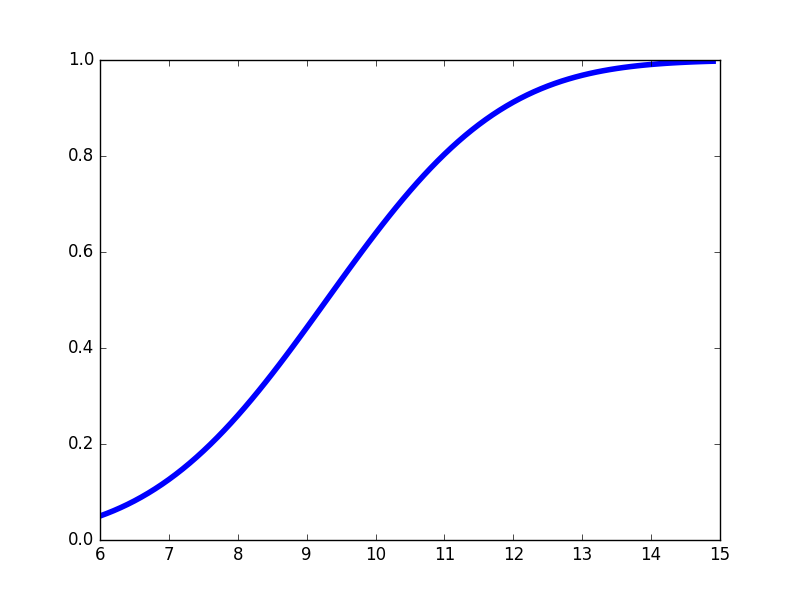
\includegraphics{power}
\caption{This function approaches 1 as $\mu_1$ approaches $\infty$.}
\end{figure}
\end{enumerate}
\end{document}
\grid
